\documentclass[12pt]{article}
\usepackage{amsmath}
\usepackage{graphicx}
\usepackage{float}
\usepackage{tabto}
\usepackage{hyperref}
\begin{document}
	\title{CS-GY 6083 B PRNCPLS DATABASE SYSTEMS Section B final project part 2 report}
	\author{Name: Siyuan Shi\\
			Net ID: ss13376\\
			Student ID: N18648680\\
			 \\
			Name: Haotian Yi\\
			Net ID: hy1651 \\
			Student ID: N18800809\\
			}
	\maketitle
	

	\newpage
	
	\section{Development Environments}
	Programming language: \href{https://www.python.org/downloads/release/python-368/}{python 3.6.8}\\
	 \\
	Web framework: \href{https://www.djangoproject.com/download/}{Django 3.0.4}\\
	 \\
	Database: \href{https://www.mysql.com/products/workbench/}{MySQL Workbench 8.0 CE}\\
	 \\
	IDE: PyCharm
	

	\subsection{Django Logic}\par
	This section introduces the logic of the project. \\\\
	(1) The first thing to do is of course create a new django project.\\\\
	(2) Then we need to connect the database to the project. This include creating authentication user for the schema, django \textit{inspectdb} command, etc. Within the django project itself, first of all, \textit{models.py} must contains all the entities that database schema contains. \\\\
	(3) \textit{settings.py} contains configuration information about database and apps created in the project. \textit{urls.py} is the root URL configuration of the project.\\\\
	(4) \textit{static} directory is used to provide our project wide static assets. \\\\
	(5) Inside \textit{views.py}, we can define Python function or class that takes a Web request and returns a Web response. \\\\
	(6) \textit{templates} directory contains all the templates the project needed. A template contains the static parts of the desired HTML output as well as some special syntax describing how dynamic content will be inserted.
	\begin{figure}[H]
		\centering
		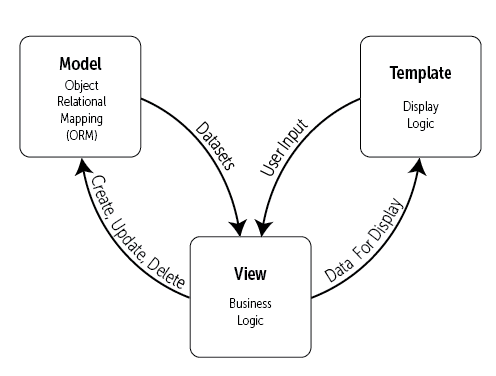
\includegraphics[scale=0.7]{django}
		\caption{Django project logic}
	\end{figure}
	Figure 2 displays the running logic of django project. Model and View is on the server side, Template is on the client side. View can be used to create, update or delete records of model. It can also provide data for display. Template is used to display data for users. Users can input data via template.
	
		\newpage
	
	\section{Database}
	\subsection{Relational Model}
	\begin{figure}[H]
		\centering
		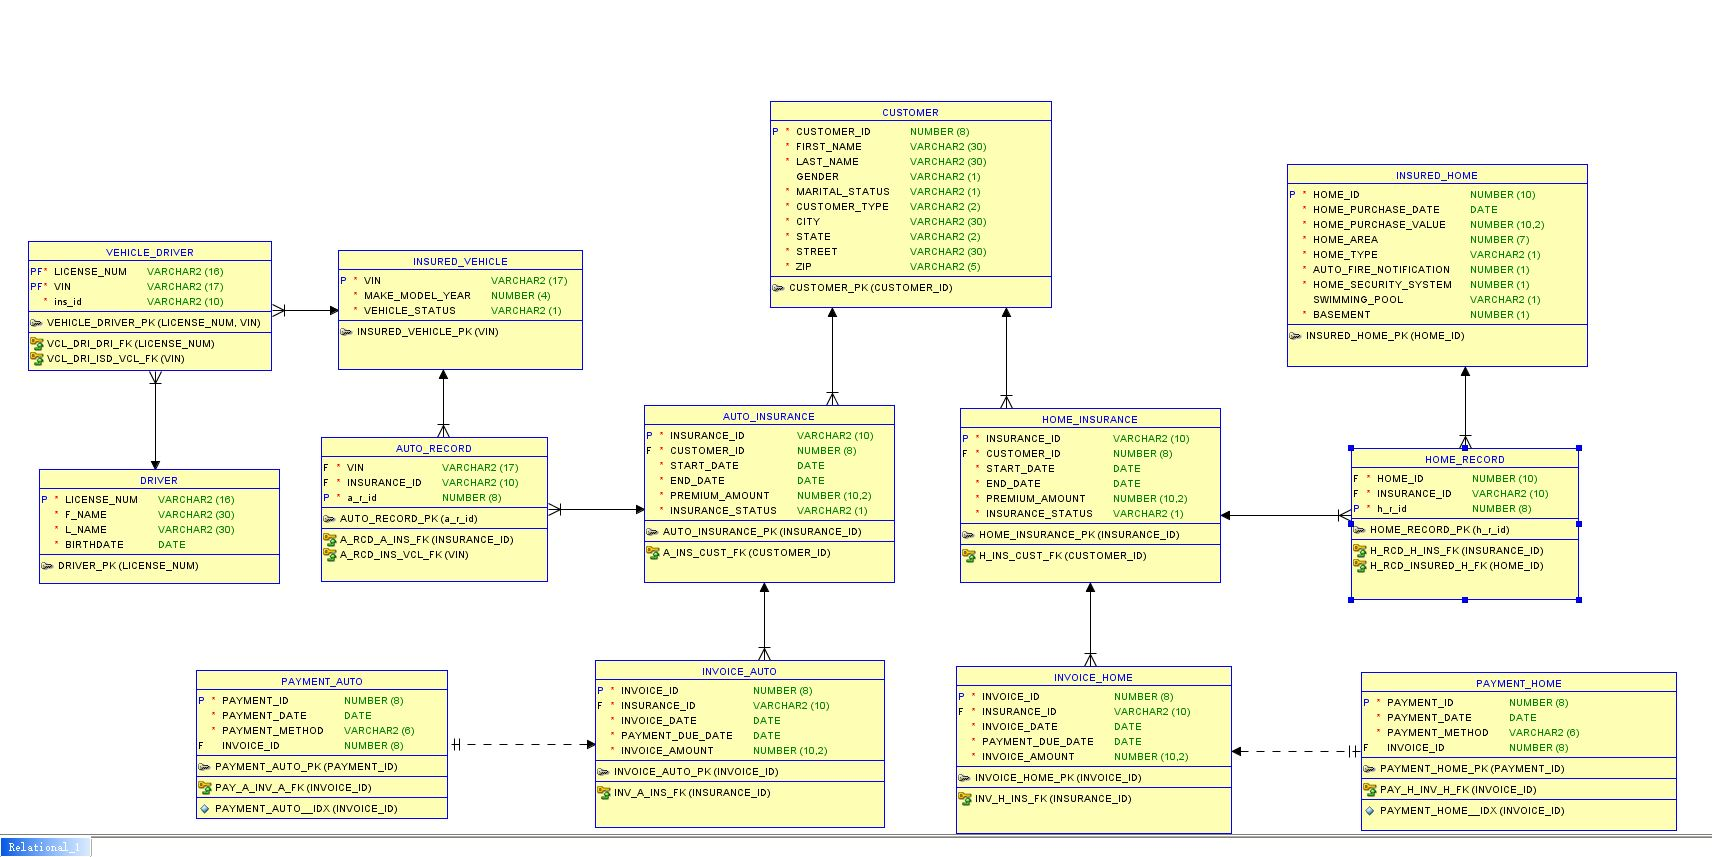
\includegraphics[scale=0.45]{rel}
		\caption{Relational Model}
	\end{figure}
	Full resolution picture of relational model is provided in a separate file.
	\newpage
		
	\subsection{DDL code}
	Here is part of DDL code:\\
	\begin{figure}[H]
		\centering
		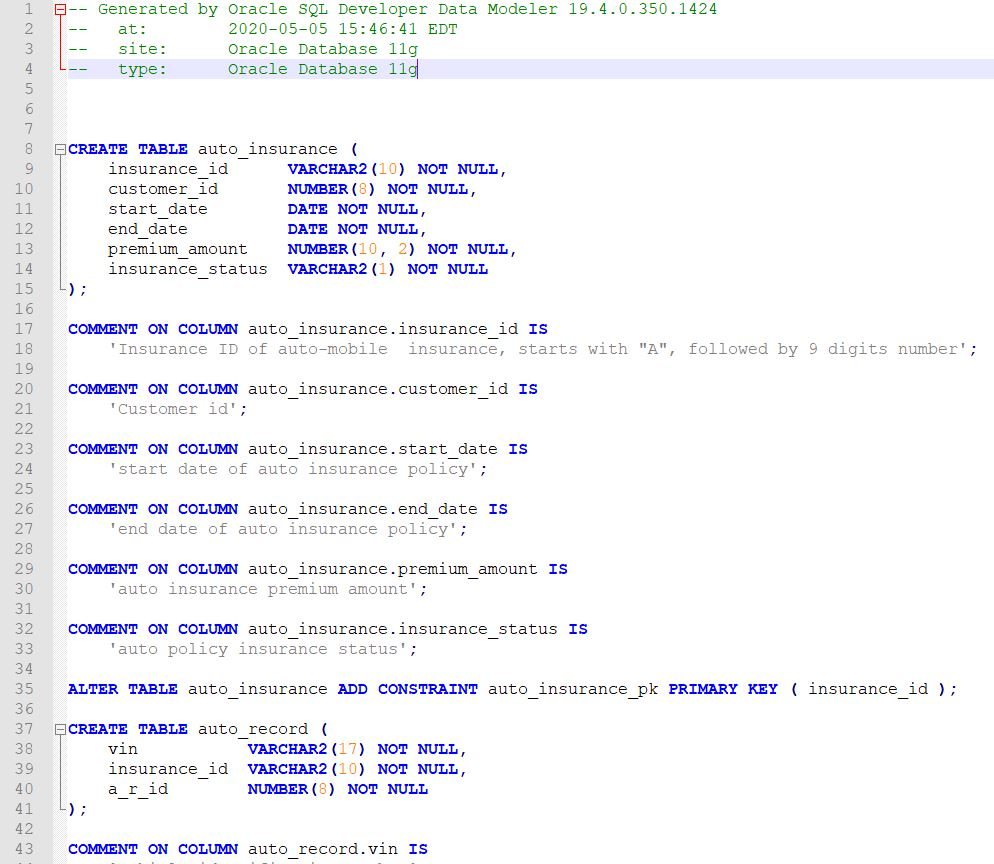
\includegraphics[scale=0.55]{ddl}
		\caption{DDL code (part)}
	\end{figure}
	Full code is provided in a separate sql file final.sql.\\
	
	\newpage
	\section{Features}
	\qquad This section depicts CRUD features and application procedure of our website.
	
	\subsection{Register, Login and Logout}
	\qquad This section introduces the sign up, login and logout feature of the project. Sign up view function will create a record in default User model with a primary key auto-created. During registering, make\_password is called so that password is encrypted using the PBKDF2 algorithm (Password-Based Key Derivation Function 2) with a SHA256 hash. When logging in, the password typed will be encrypted and send to server. After logout, the session data for the current request is completely cleaned out.\\
	\begin{figure}[H]
		\centering
		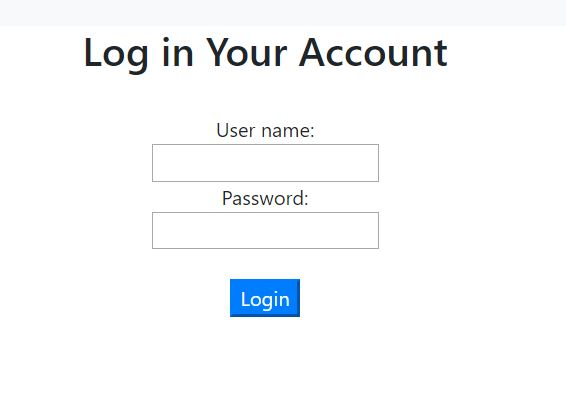
\includegraphics[scale=0.8]{login}
		\caption{Login}
	\end{figure}
	\begin{figure}[H]
		\centering
		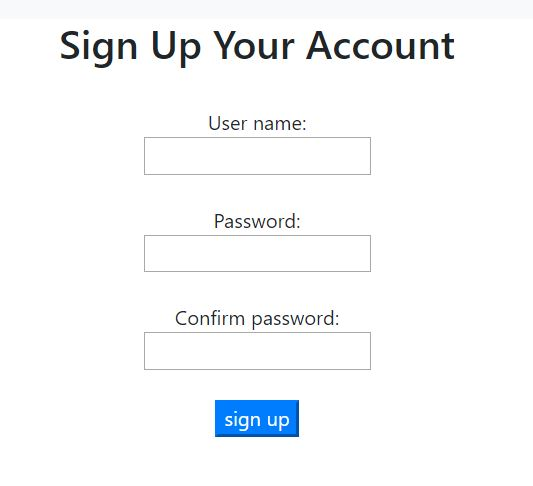
\includegraphics[scale=0.6]{register}
		\caption{Sign up}
	\end{figure}
	
	
	
	\subsection{Update | Personal Center}  
	\qquad This section introduces the update feature of the project. A user can update personal information displayed in personal center. Insurance related information can also be modified, however, this operation is reserved for administrator.\\
	\begin{figure}[H]
		\centering
		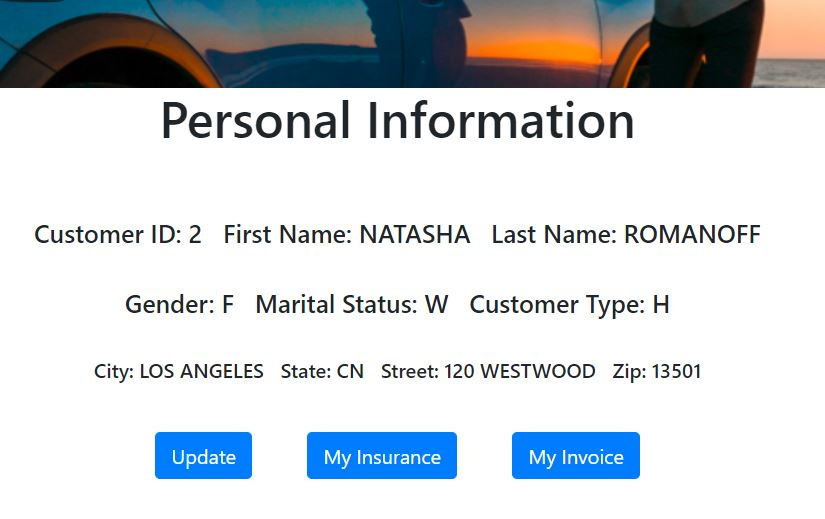
\includegraphics[scale=0.6]{per}
		\caption{Personal Center}
	\end{figure}
	\newpage
	\begin{figure}[H]
		\centering
		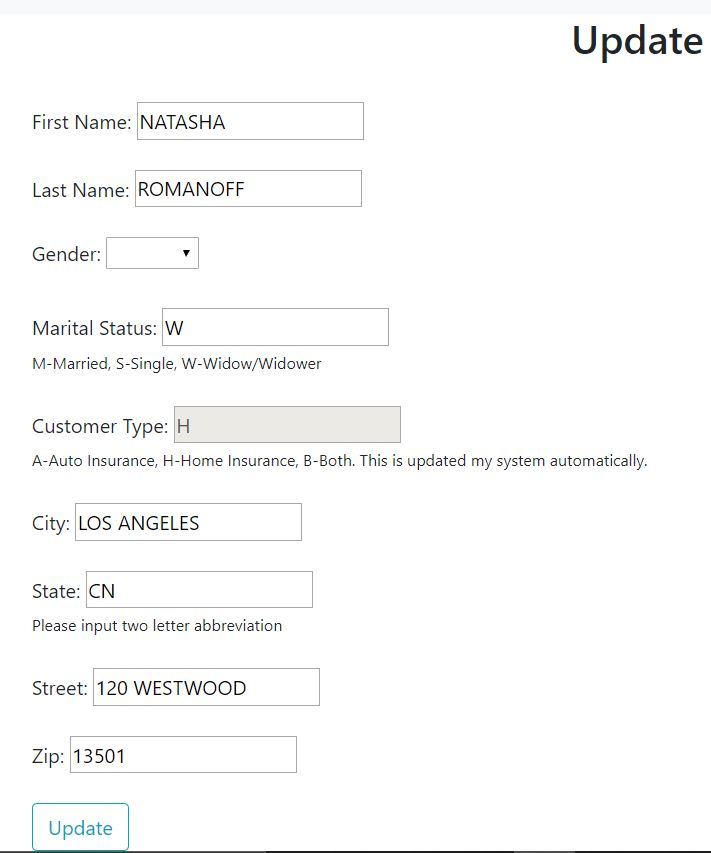
\includegraphics[scale=0.8]{updateinfo}
		\caption{Update Info}
	\end{figure}
	\newpage
	
	
	\subsection{Insert | Purchase}
	\qquad This section introduces the insert feature of the project. After user purchase an insurance, necessary records will be inserted into different tables of the database. Take home insurance for example:\\\\
	(1) Start page for home insurance:
	\begin{figure}[H]
		\centering
		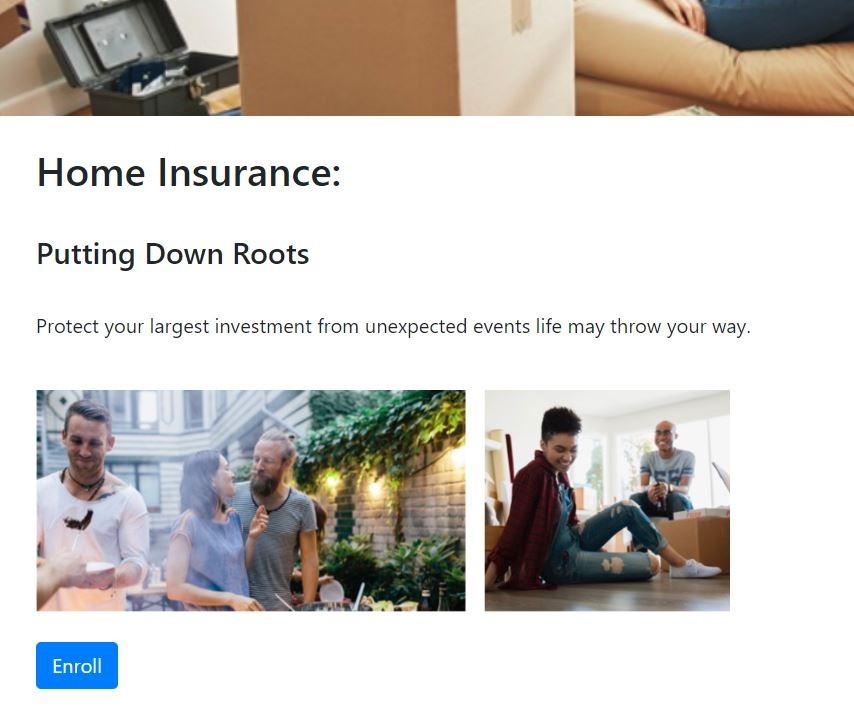
\includegraphics[scale=0.7]{hins}
		\caption{Start page}
	\end{figure}
	\newpage
	\noindent(2) Fill insurance information:
	\begin{figure}[H]
		\centering
		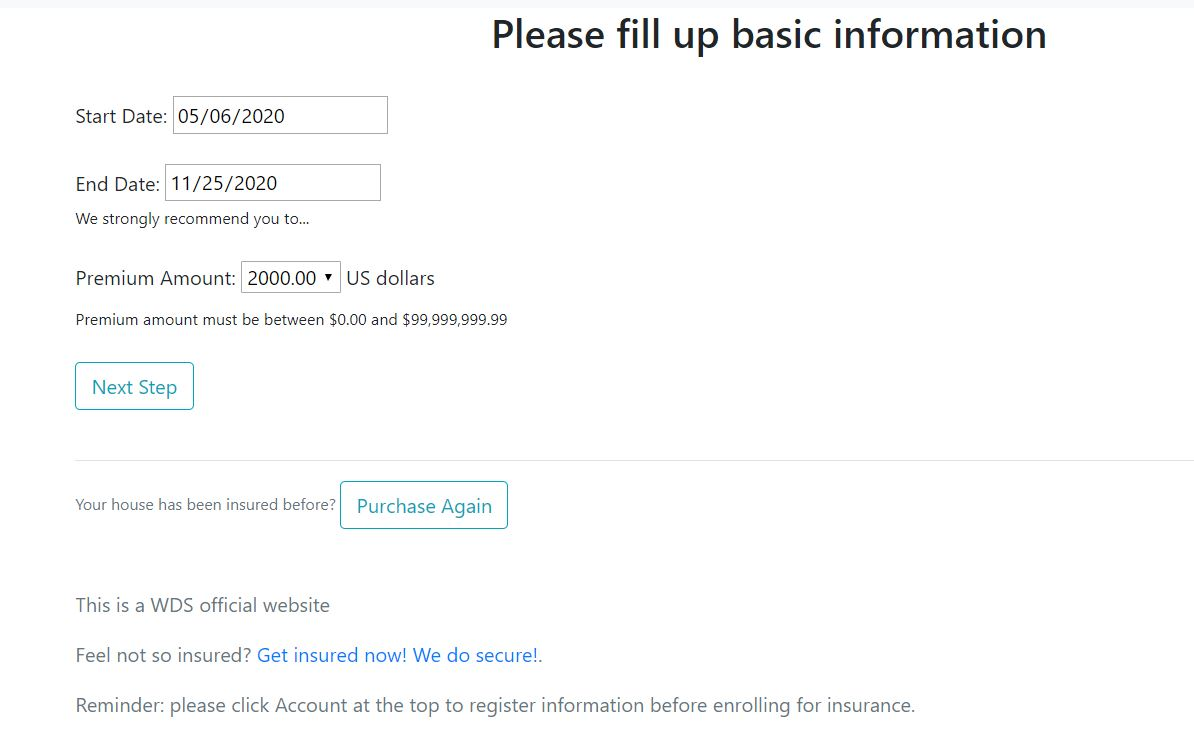
\includegraphics[scale=0.7]{homeinsurance}
		\caption{Home Insurance}
	\end{figure}
	\newpage
	\noindent(3) Start date cannot be earlier than today:
	\begin{figure}[H]
		\centering
		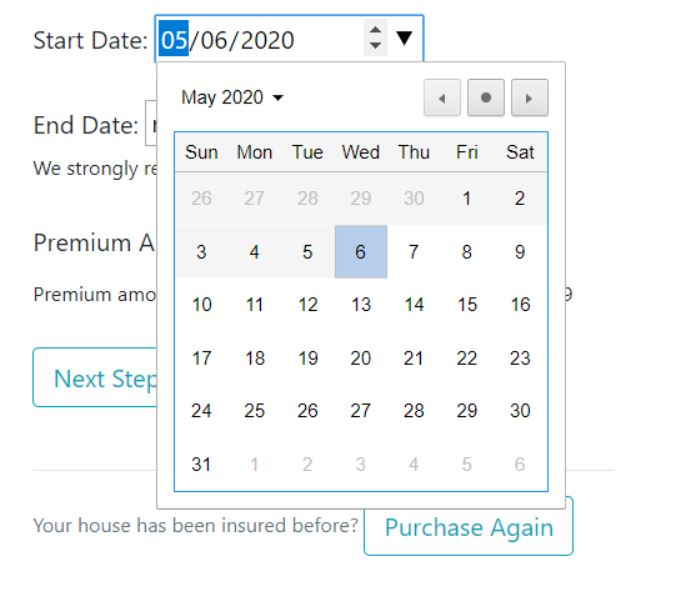
\includegraphics[scale=0.56]{startdatejquery}
		\caption{Start date restriction}
	\end{figure}
	\noindent(4) End date chosen by option:
	\begin{figure}[H]
		\centering
		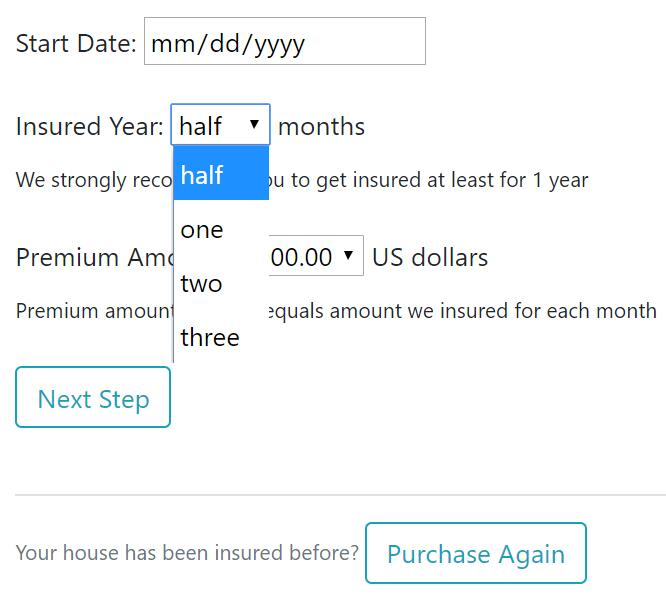
\includegraphics[scale=0.5]{enddatejquery}
		\caption{End date restriction}
	\end{figure}
	\noindent (5) Fill up insured home information:
	\begin{figure}[H]
		\centering
		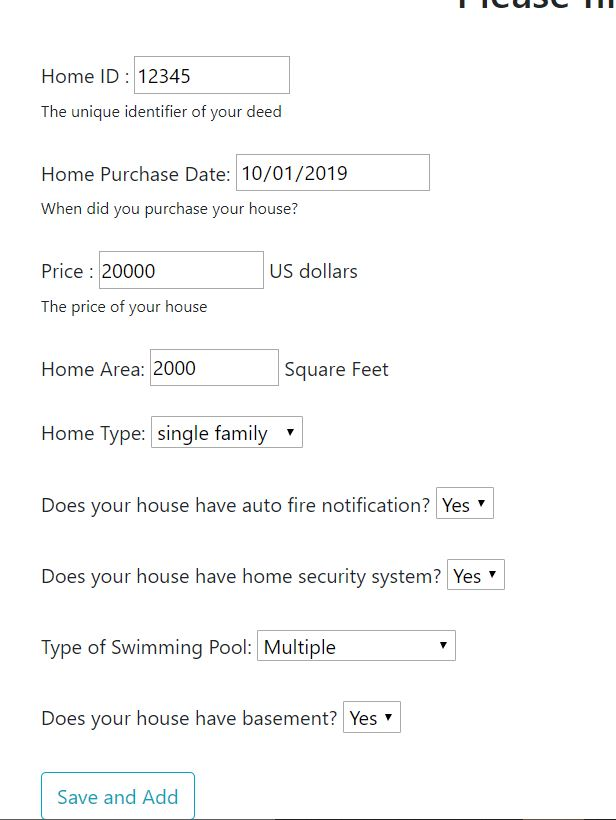
\includegraphics[scale=0.58]{insuredhome}
		\caption{Insured Home}
	\end{figure}
	\noindent(6) View order information and pay:
	\begin{figure}[H]
		\centering
		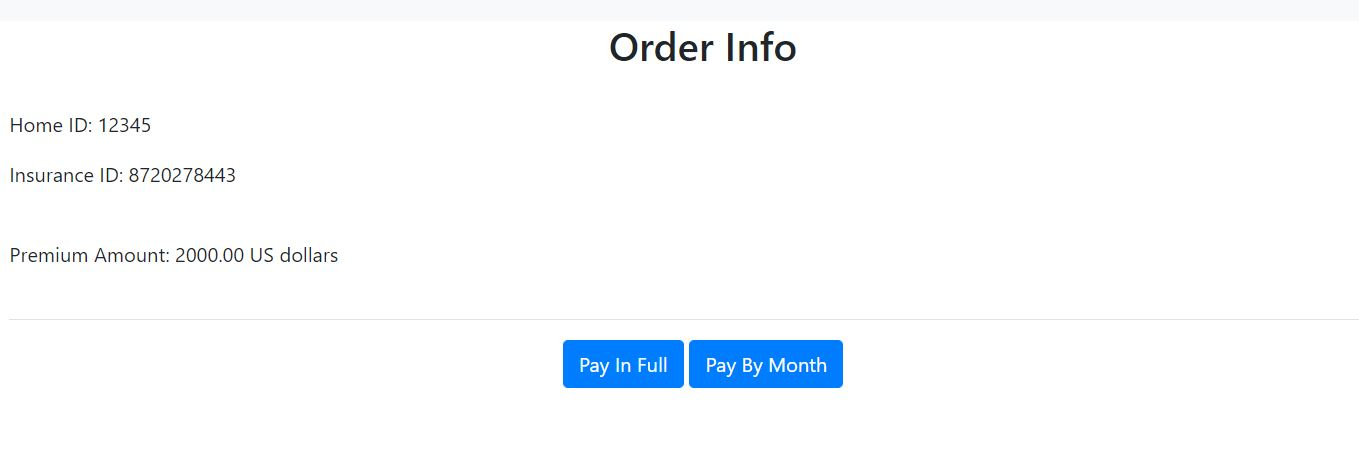
\includegraphics[scale=0.52]{orderinfo}
		\caption{Order Info}
	\end{figure}
	\noindent (7) View invoice:
	\begin{figure}[H]
		\centering
		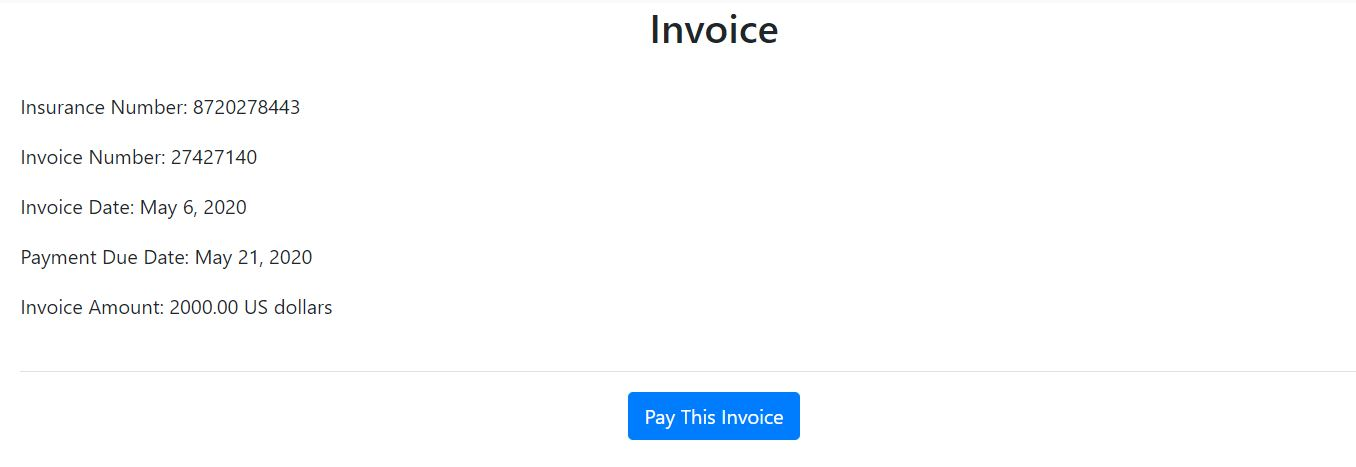
\includegraphics[scale=0.52]{invoice}
		\caption{Invoice}
	\end{figure}
	\noindent (8) Make payment:
	\begin{figure}[H]
		\centering
		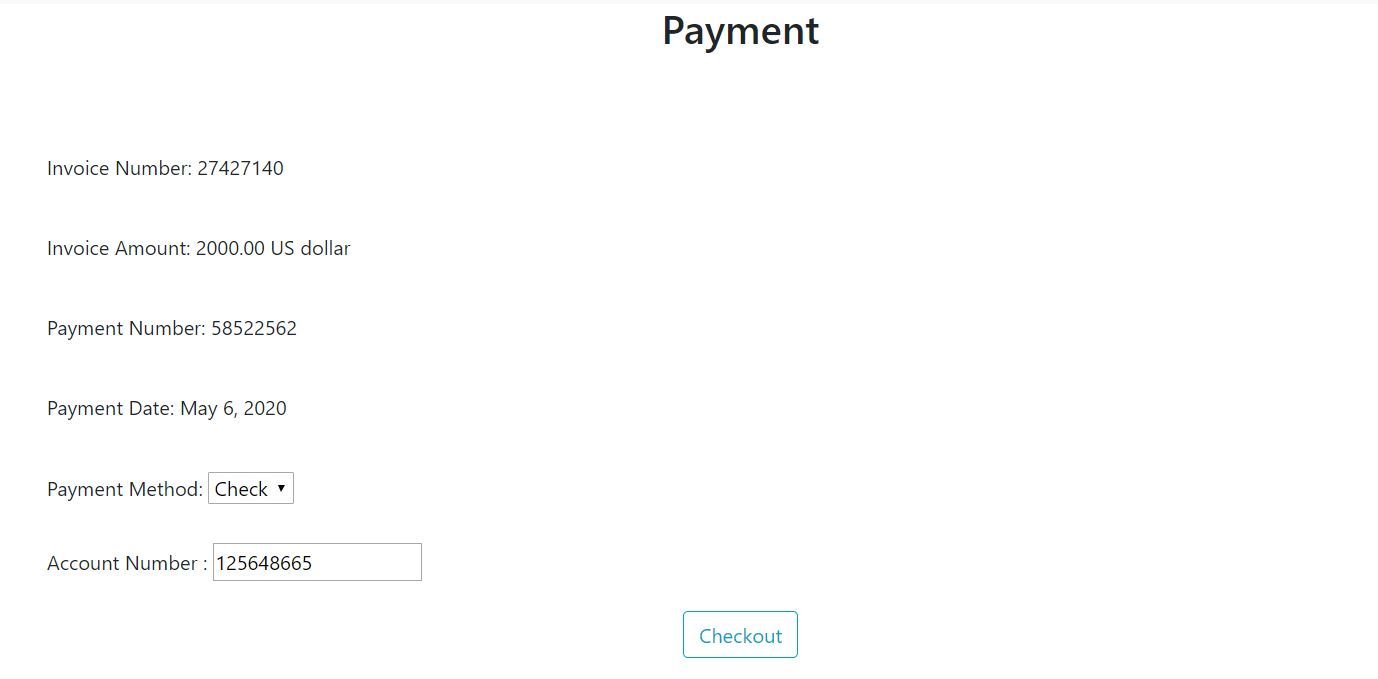
\includegraphics[scale=0.58]{payment}
		\caption{Payment}
	\end{figure}
	
	\newpage
	
	\subsection{Query | Insurance,Invoice \& Payment}
	\qquad This section introduces the query feature of the project. There are two kinds of query in this project, insurance query and invoice query. Insurance query consists of home insurance query and auto insurance query. User can only query on his or her own data, including insurance information, house information, vehicle information, driver information, etc. Invoice query is used for displaying user's invoices. User can also use this entrance to pay installment invoices.\\\\
	\noindent (1) Query Insurance information:
	\begin{figure}[H]
		\centering
		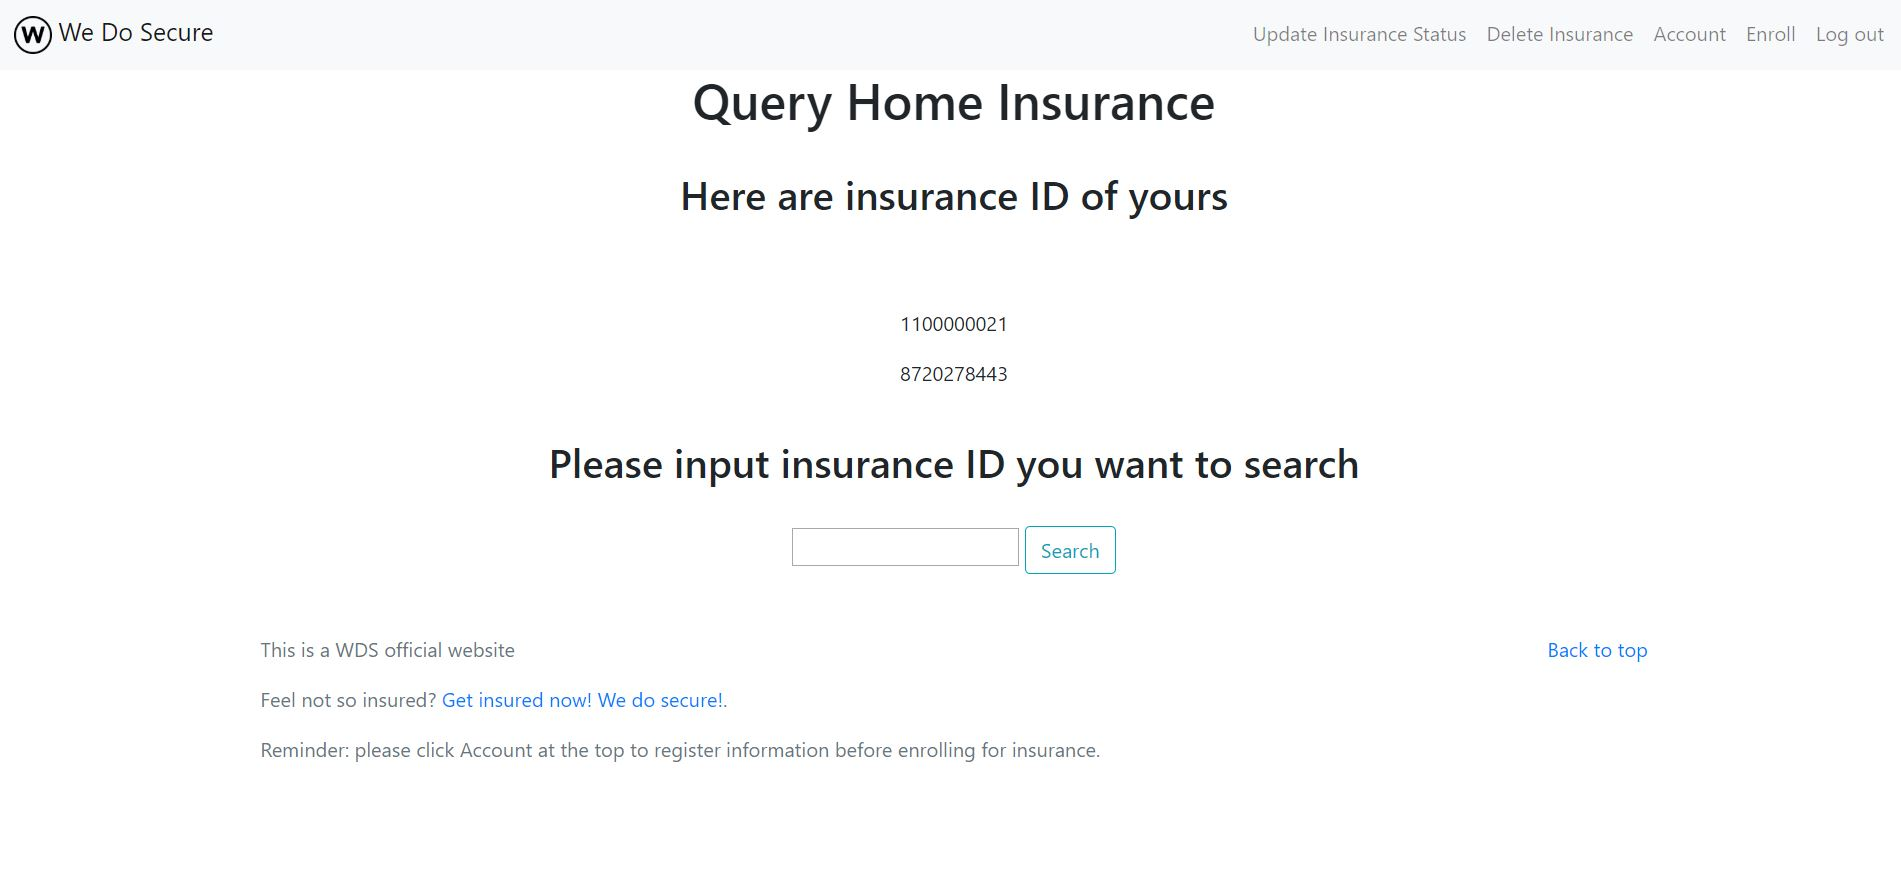
\includegraphics[scale=0.35]{homeinsurancequery}
		\caption{Home Insurance Query}
	\end{figure}
	\begin{figure}[H]
		\centering
		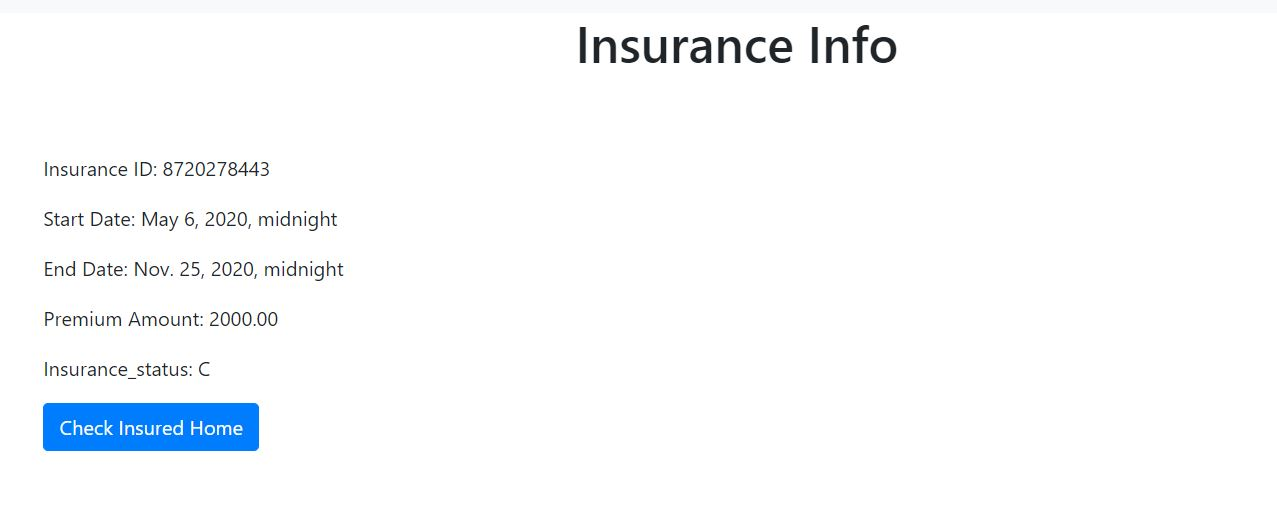
\includegraphics[scale=0.4]{insurinfo}
		\caption{Home Insurance Info}
	\end{figure}
	\begin{figure}[H]
		\centering
		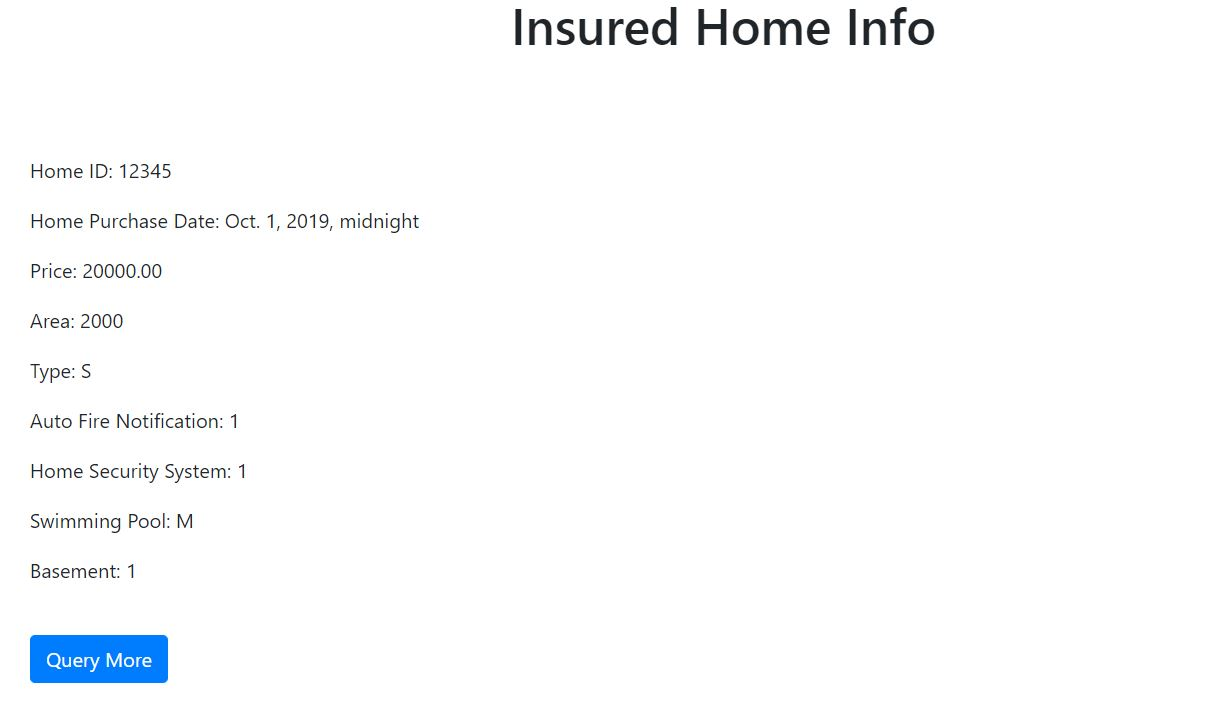
\includegraphics[scale=0.4]{homeinfo}
		\caption{Home Info}
	\end{figure}
    \noindent (2) Query invoice and payment: this is designed for users to check all their invoice details and pay installment. iF one choose to pay installments, there will be multiple invoice for one insurance.\\
	\begin{figure}[H]
		\centering
		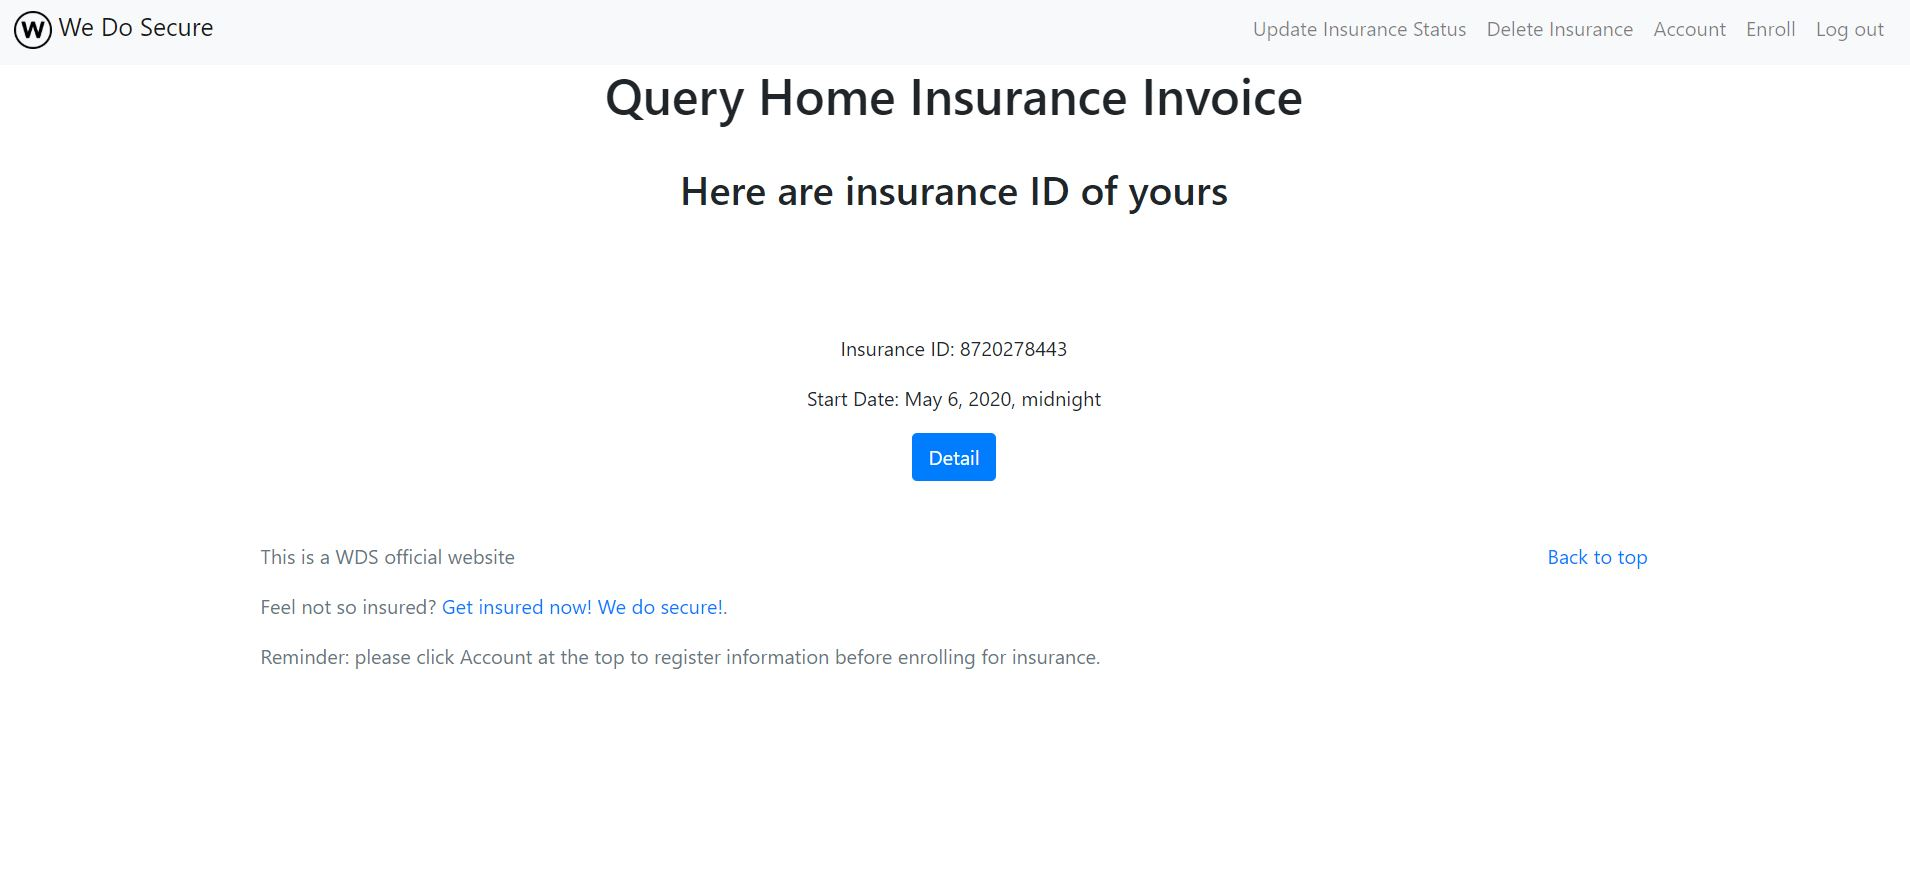
\includegraphics[scale=0.38]{homeinvoicequery}
		\caption{Home Invoice Query}
	\end{figure}
	\begin{figure}[H]
		\centering
		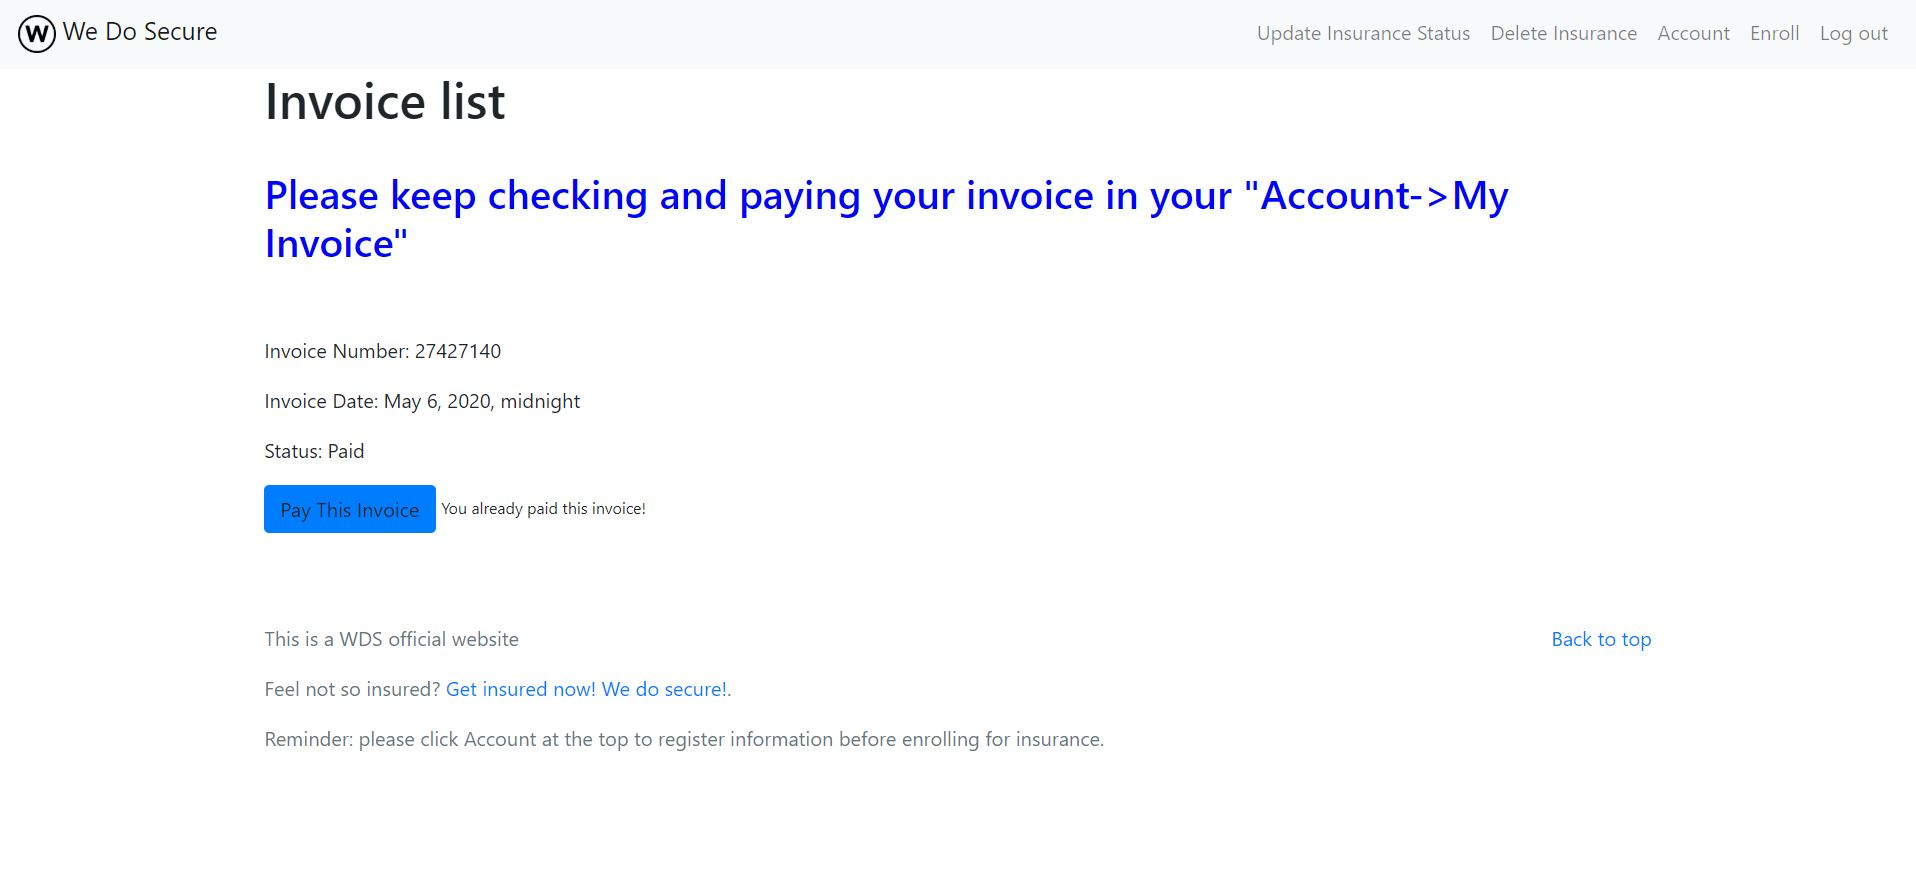
\includegraphics[scale=0.38]{homeinvoicequeryresult}
		\caption{Home Invoice Query Result}
	\end{figure}

	
	\subsection{Delete | Superuser Function}
	This section introduces the delete feature of the project. Delete feature is designed for administrator. An administrator can delete a certain insurance record and all related information.\\\\
	\noindent (1) Input insurance ID to delete:
	\begin{figure}[H]
		\centering
		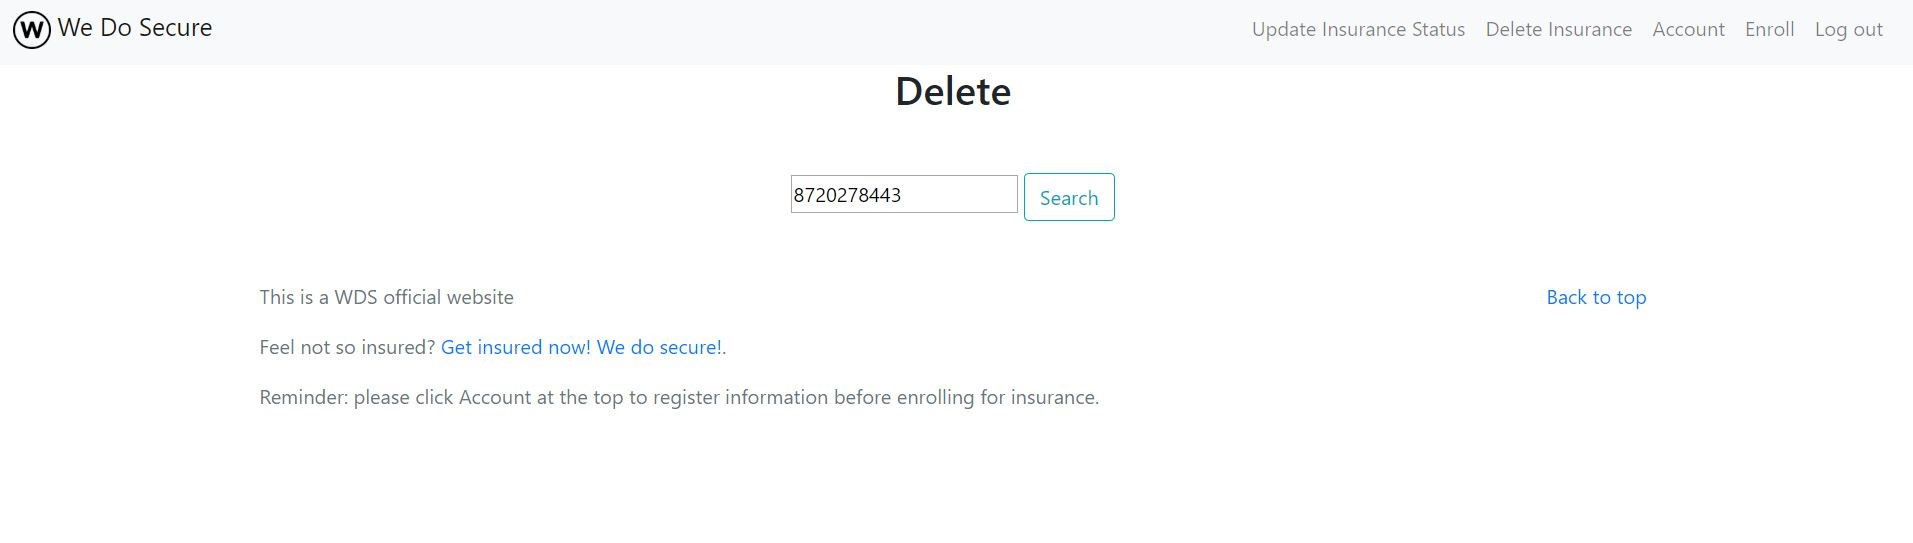
\includegraphics[scale=0.38]{delete}
		\caption{Delete}
	\end{figure}
    \newpage
    \noindent (2) Confirm delete:
	\begin{figure}[H]
		\centering
		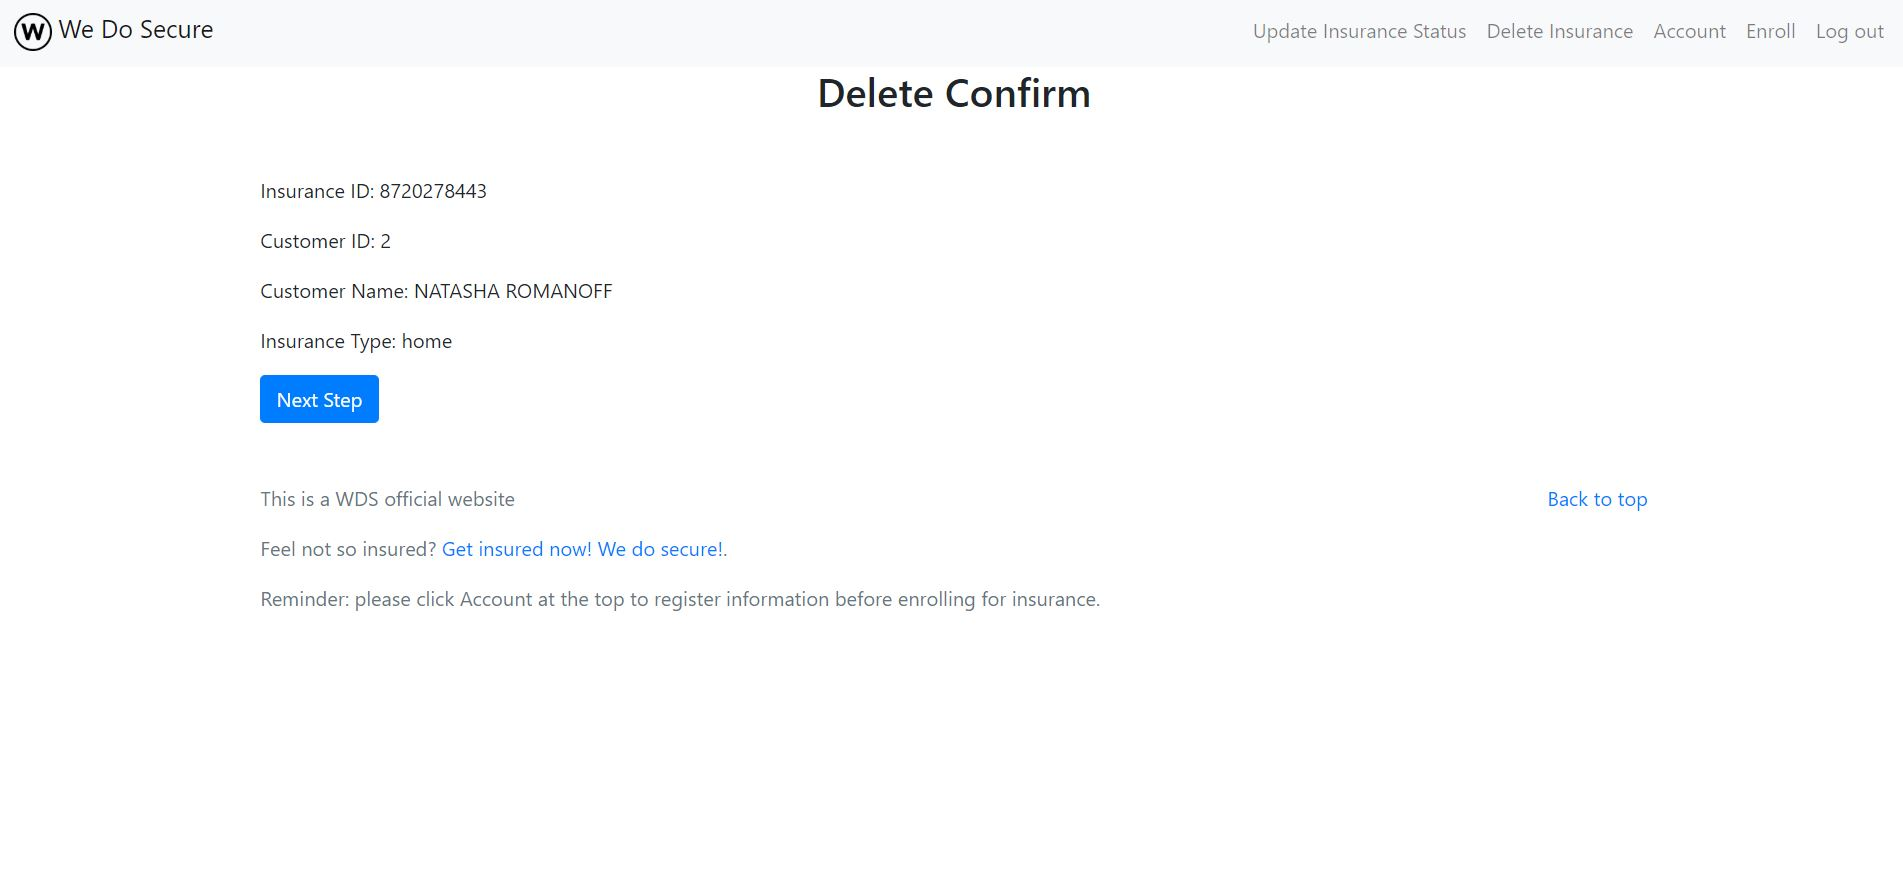
\includegraphics[scale=0.38]{deleteconfirm}
		\caption{Delete Confirm}
	\end{figure}
	\noindent (3) Click to delete and lift result message:
	\begin{figure}[H]
		\centering
		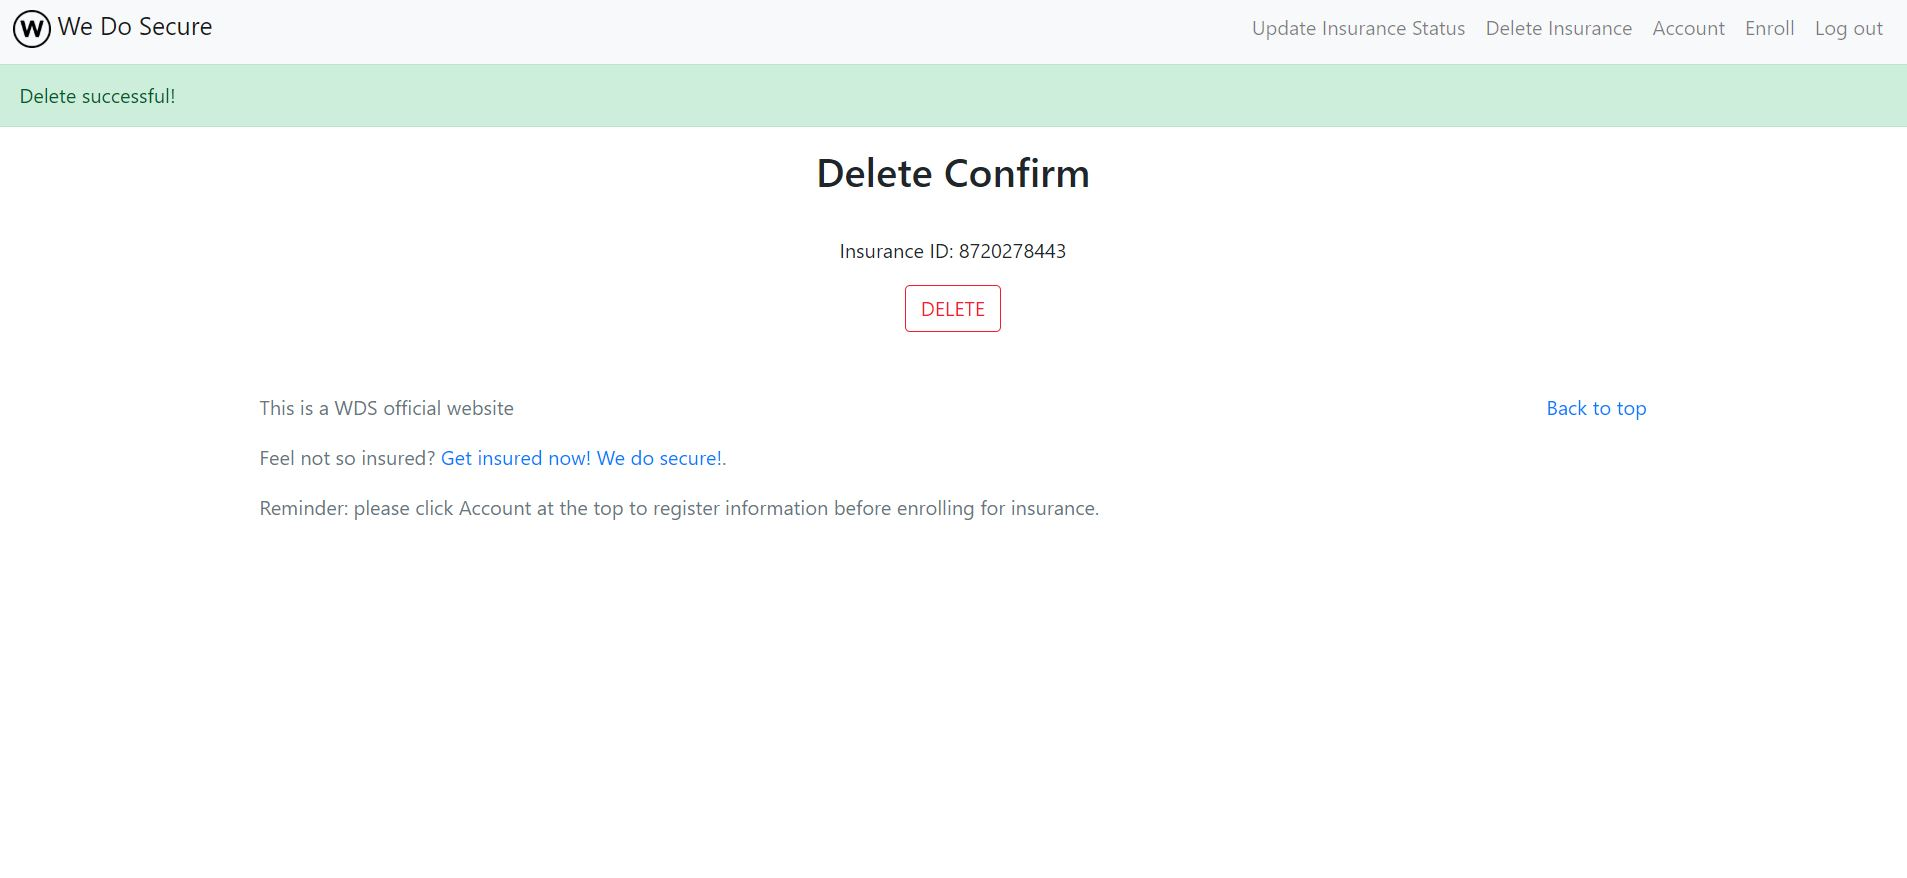
\includegraphics[scale=0.38]{deleteresult}
		\caption{Delete Result}
	\end{figure}
	
	
	
	\subsection{Extra Feature Summary}
	\textbf{(1) Index}
	\begin{figure}[H]
		\centering
		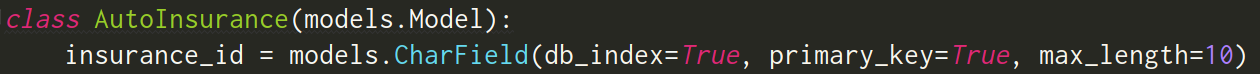
\includegraphics[scale=0.3]{index.png}
		\caption{Index}
	\end{figure}
	For the index feature, we follow the thumb rule that we build index on attributes that are frequently queried. In Django, it is easy to enable index feature, with the statement \textit{db\_index=Ture} above, it builds a B+ tree index on the attribute.
    \\\\
    \noindent\textbf{(2) Password encryption}
    \begin{figure}[H]
    	\centering
    	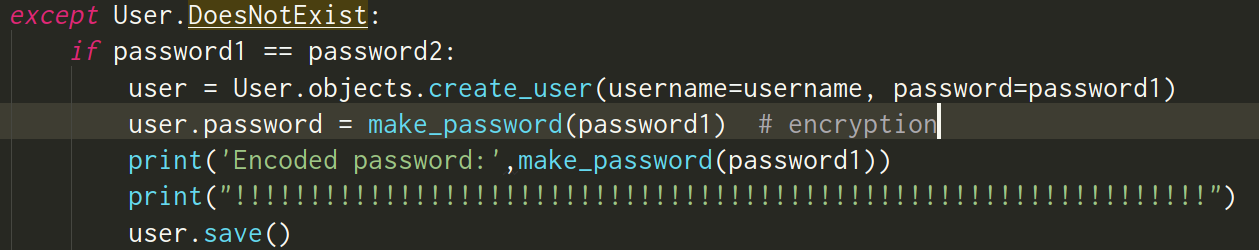
\includegraphics[scale=0.3]{encryption.png}
    	\caption{Encryption}
    \end{figure}
    After create user, change password attribute by using \textit{make\_password()} to encrypt. Then use \textit{auth.authenticate()} below to authenticate users to login.
    \begin{figure}[H]
    	\centering
    	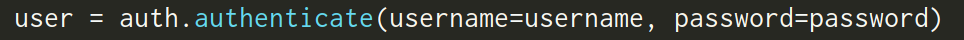
\includegraphics[scale=0.4]{authenticate.png}
    	\caption{Authenticate}
    \end{figure}

    \newpage
    \noindent\textbf{(3) CSRF}
    \begin{figure}[H]
    	\centering
    	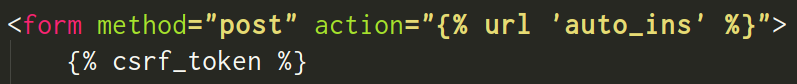
\includegraphics[scale=0.49]{csrf.png}
    	\caption{CSRF}
    \end{figure}
    Add \textit{ \{\% csrf\_tocken \%\} } to get protection from CSRF (Cross Site Request Forgery) attack.\\
	
	\noindent\textbf{(4) Status Update (automatic)}
	\begin{figure}[H]
		\centering
		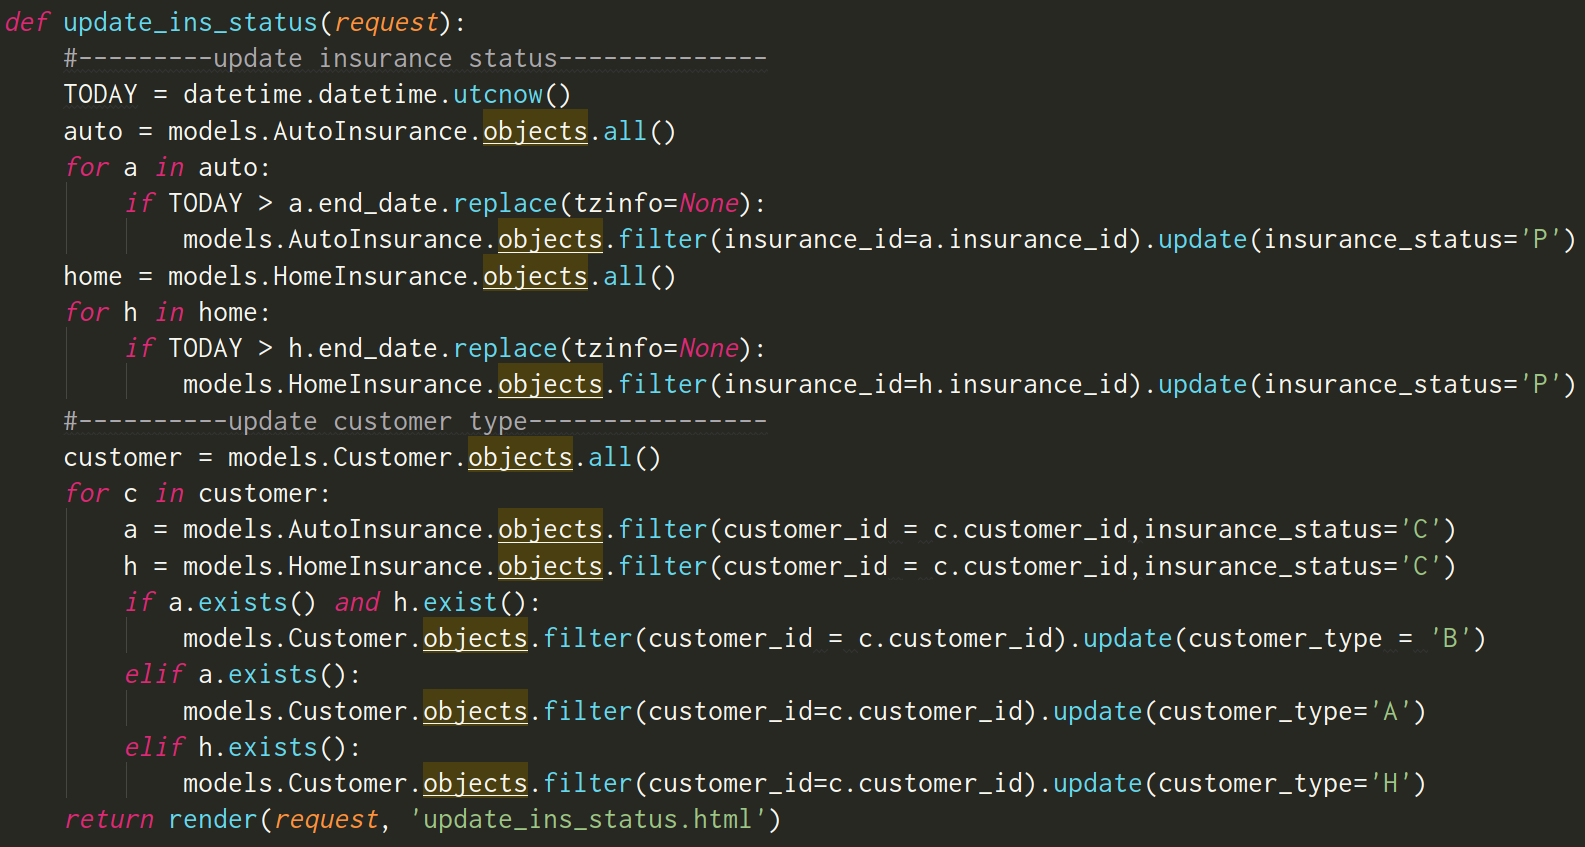
\includegraphics[scale=0.25]{update.png}
		\caption{Status Update}
	\end{figure}
	Achieve a function for superuser to update insurance status and customer type, also, this update function is embedded in personal center (interface to view related information), every time a user access personal center, it will automatically update status of current user.
	
	\newpage
	\noindent\textbf{(5) SQL Injection}
	\begin{figure}[H]
		\centering
		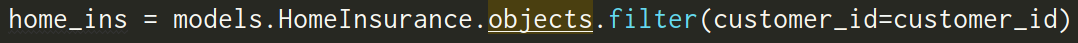
\includegraphics[scale=0.36]{injection.png}
		\caption{SQL Injection}
	\end{figure}
	In the aspect of SQL Injection, we prevent this by using Django ORM function, it process input by only accepting value for corresponding attribute, thus protect from injection.\\
    
    \noindent\textbf{(6) jQuery}
    \begin{figure}[H]
    	\centering
    	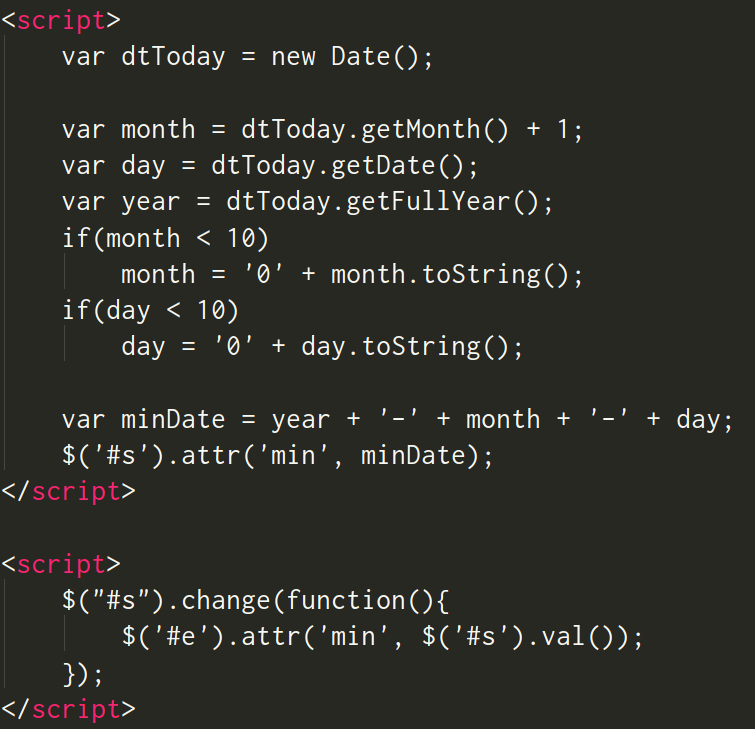
\includegraphics[scale=0.32]{jquery.png}
    	\caption{jQuery}
    \end{figure}
    When designing template for home insurance and auto insurance, we use jQuery to dynamically set attribute for certain input tag (start date) so that user cannot choose a date before today as the start date for home or auto insurance. We also use option to restrict end date such that user cannot choose a date earlier than start date. These restrictions for input is essential for the stable of database.
    
    \newpage
    \noindent\textbf{(7) Beautified UI}\\\par
    Figures below are UI sample we beautified by HTML, CSS, bootstrap templates. 
    \begin{figure}[H]
    	\centering
    	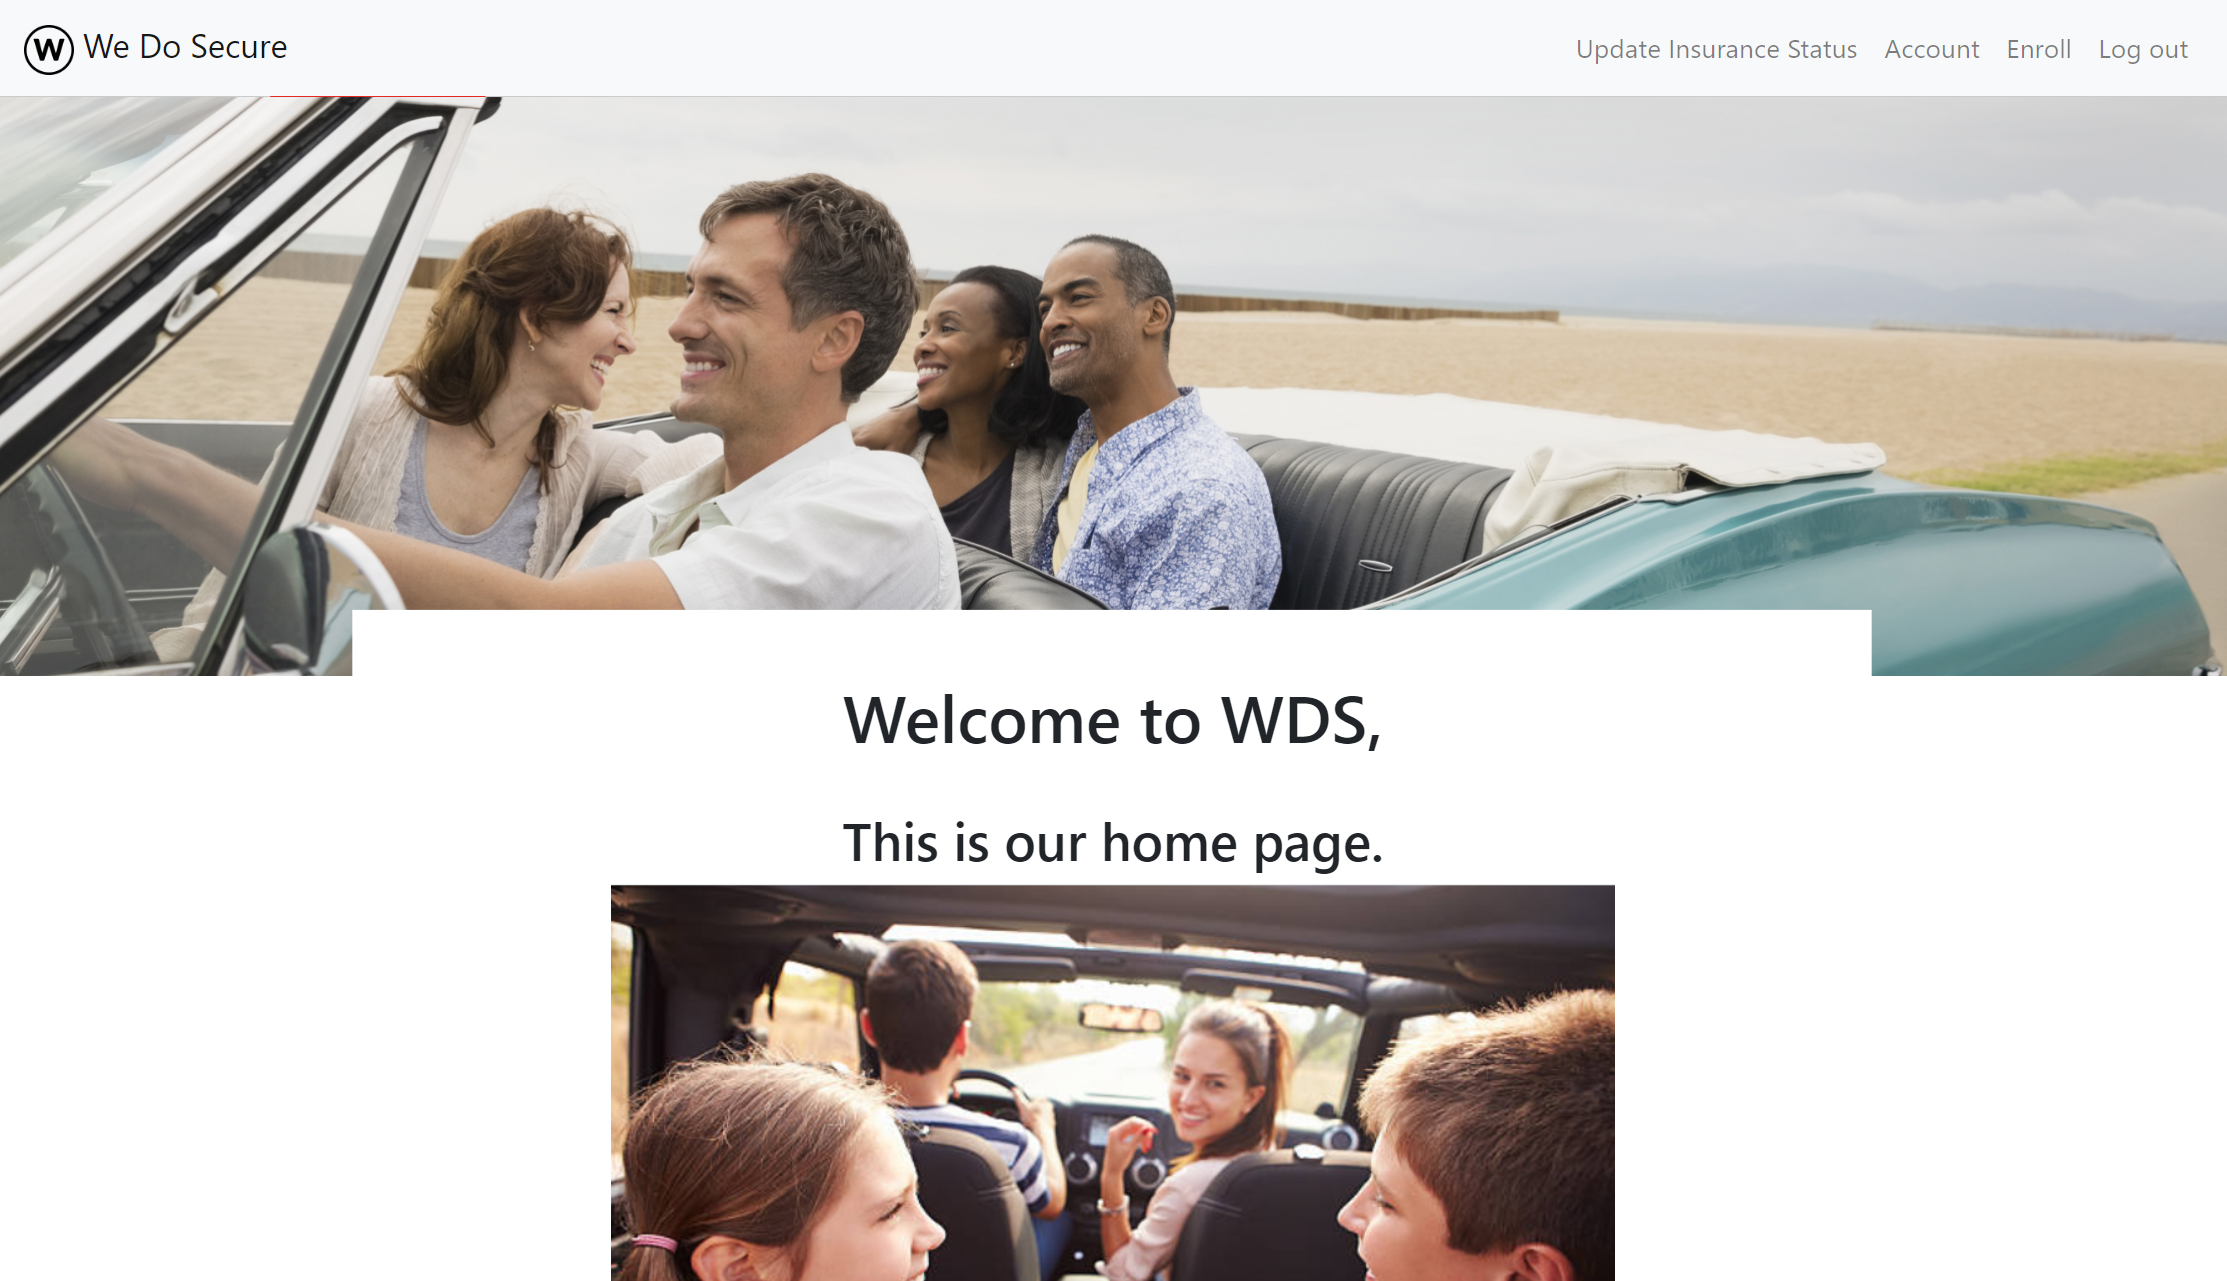
\includegraphics[scale=0.09]{ui.png}
    	\caption{UI sample -1}
    \end{figure}
    \begin{figure}[H]
    	\centering
    	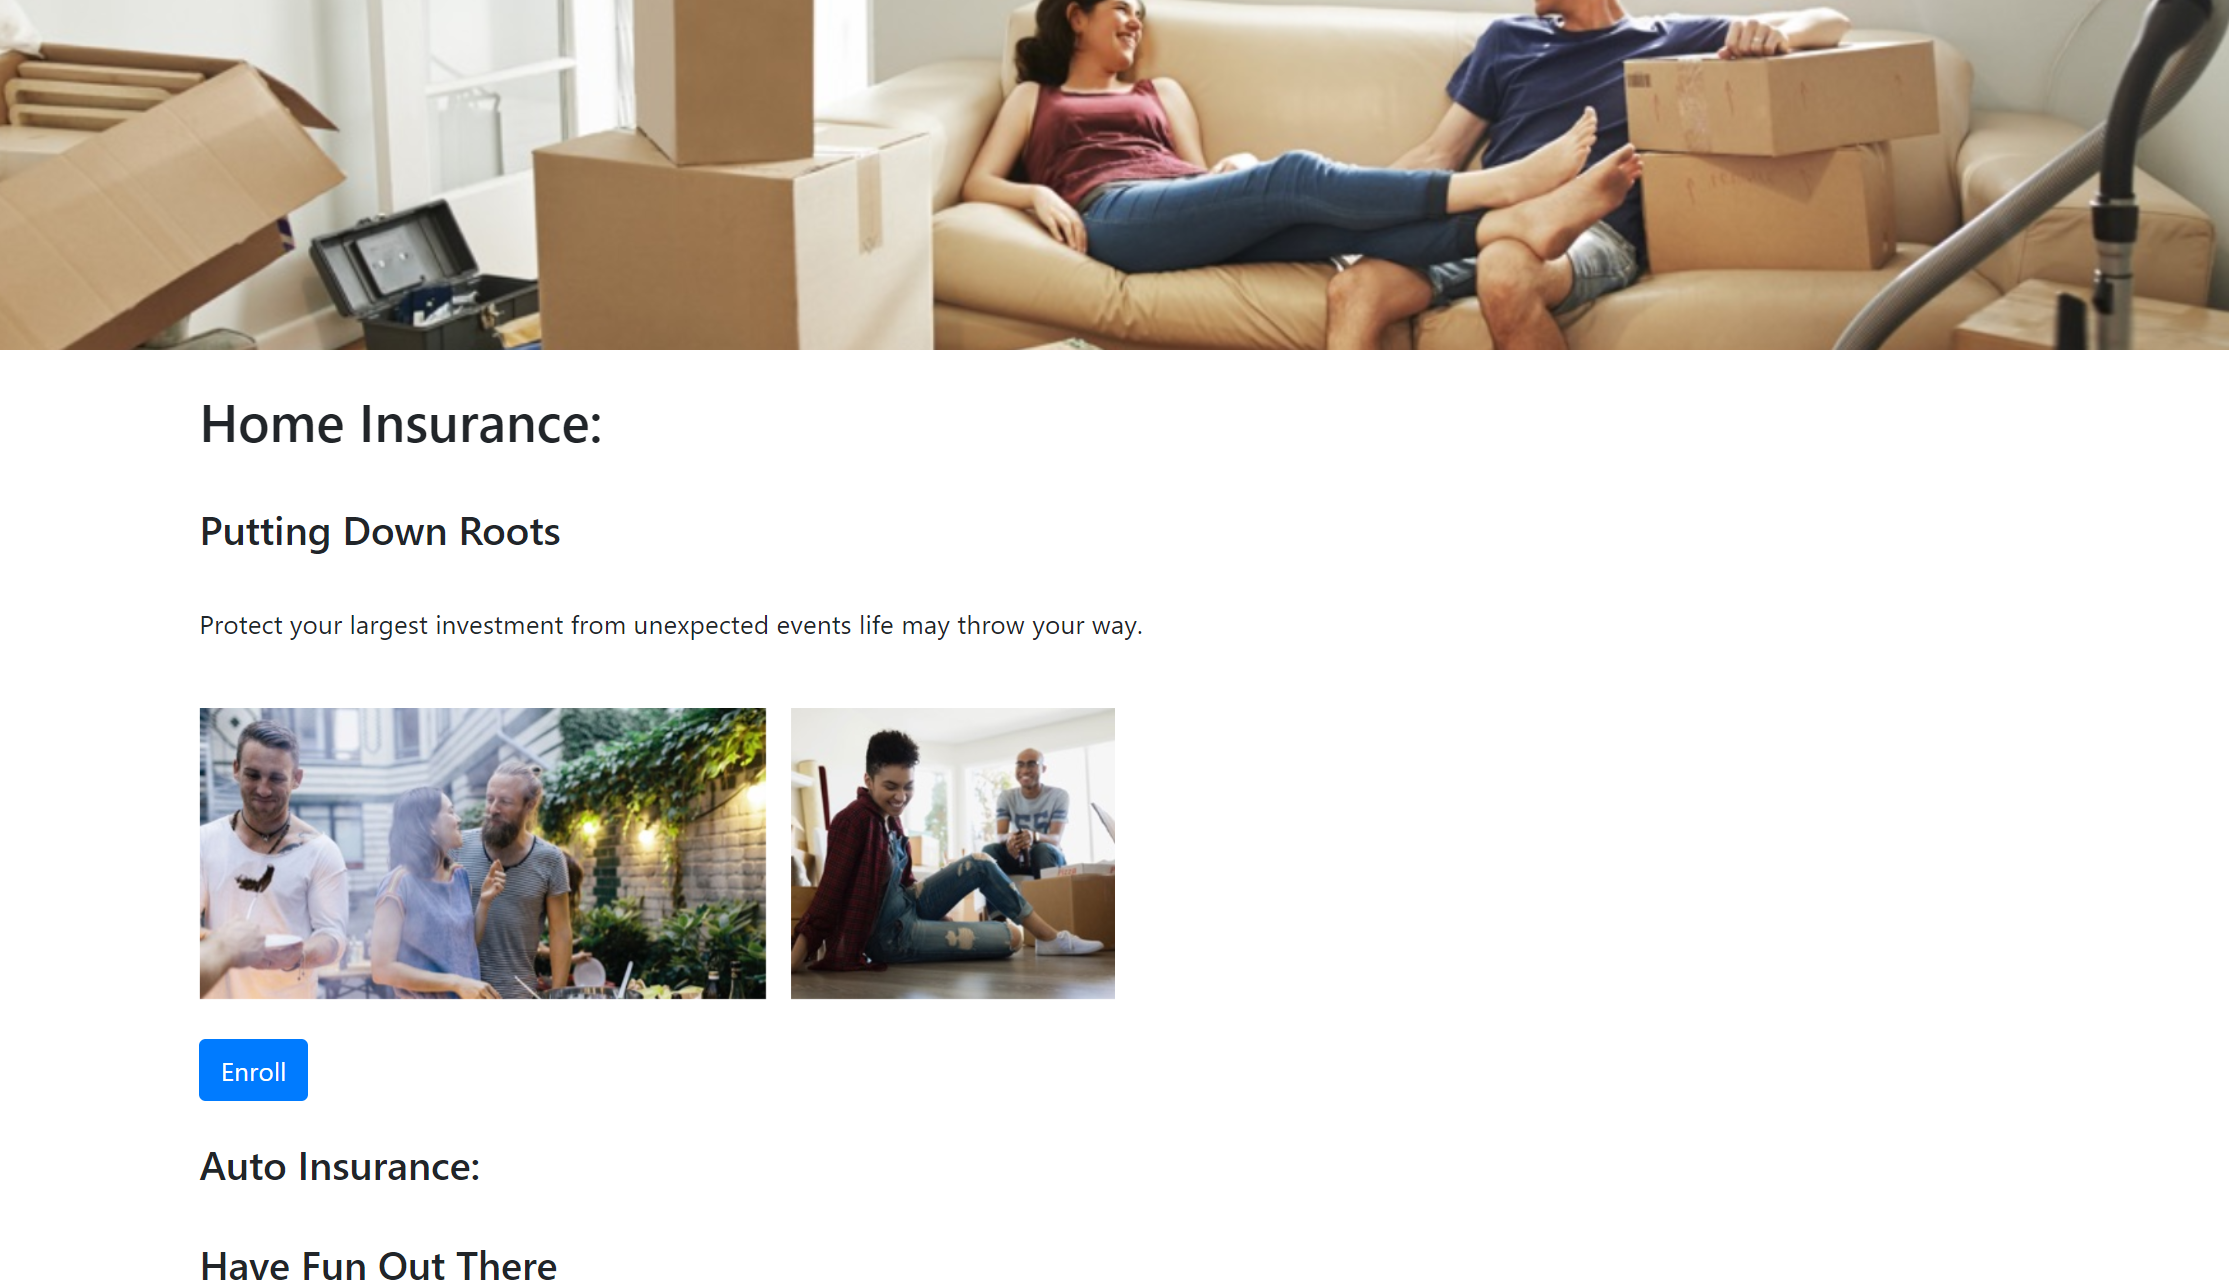
\includegraphics[scale=0.09]{ui1.png}
    	\caption{UI sample -2}
    \end{figure}
	\begin{figure}[H]
		\centering
		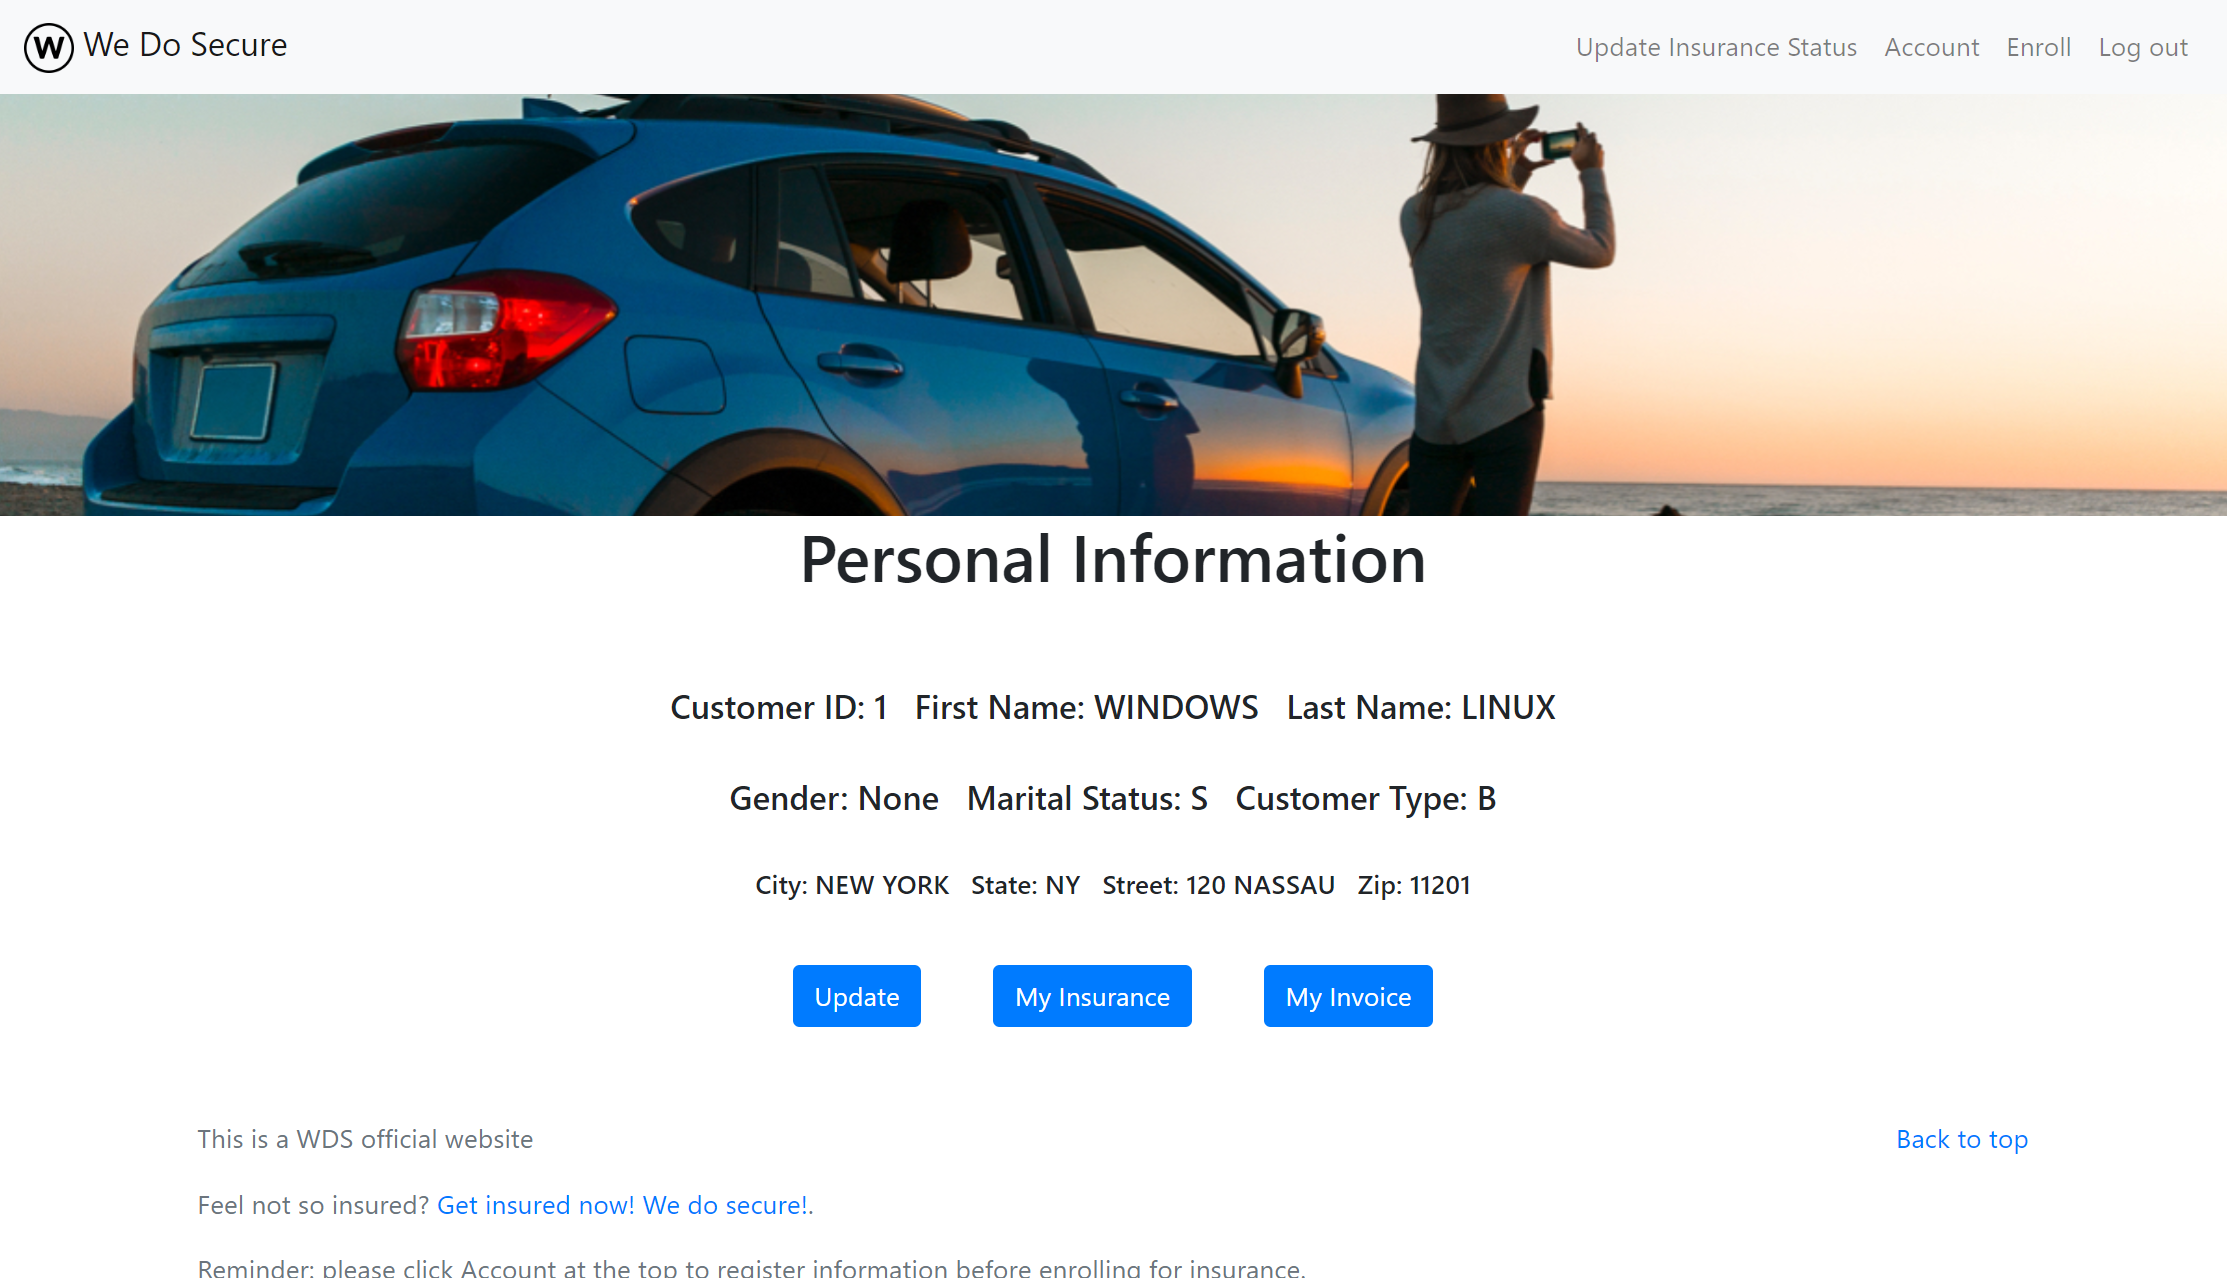
\includegraphics[scale=0.09]{ui2.png}
		\caption{UI sample -3}
	\end{figure}
    
	\section{Learning Outcome}
	\textbf{(1) About input constraint}\\\par
	When considering about input for a practical website, we have to think about constraints, that doesn't mean we let invalid input trigger error in database, we should validate input at web page and lift reminder once a input is invalid.\\\par
	Also we have to consider correlation between inputs like start date and end date, so we used jquery to limit selection of date.\\\\
	\textbf{(2) About passing argument}\\\par
	In this project, we used different ways to passing argument. Argument can be passed via render or redirect function. We can also use \textit{href} attribute in html file to achieve redirecting with parameters. Another way is to store variables using \textit{session} such that other function can use the stored variables in the same session.\\\\
	\textbf{(3) About procedure of design}\\\par
	After this project, we are more familiar with the procedure of building a website and its application, especially we feel that we must be careful when design a conceptual model for business and database because a good design can really save time in building website page and alteration for logic mistakes.
	Moreover, we think there will always be problems we can't predict when designing database models in advance but encounter in practice.
	
	\section{Other}
	We changed our model in part i.\\
	1. We add home record ID and auto record ID in HomeRecord and AutoRecord respectively.\\
	2. We add insurance id attribute to VehicleDriver. Because the same vehicle and driver may be assigned to many insurances.
	
	
	
\end{document}